
\documentclass[journal]{IEEEtran}
\usepackage{graphicx}
\usepackage{float}
\usepackage[scriptsize,labelformat=empty]{caption}
\usepackage[nodisplayskipstretch]{setspace}
\setstretch{1.25}

\renewcommand{\arraystretch}{1.1}
\begin{document}

% Don't change this portion-- it will format the section below for you.:)
\newcommand{\labtitlepage}{
	\onecolumn
	\thispagestyle{empty} \vspace*{\fill}
	\begin{center}
		\LARGE\labtitle \\ \bigskip \bigskip \large\name \\ \bigskip
		\labsection \\ \bigskip \labdate 
	\end{center}
	\vspace*{\fill} \vspace*{\fill} \newpage
	\setcounter{page}{1}
	\twocolumn
}

%% Change these variables
\newcommand{\labtitle}{CSM152A Lab 3: Stopwatch}
\newcommand{\name}{Jonathan Hurwitz 804258351 \\ Ram Sivasundaram 704261325}
\newcommand{\labsection}{Lab Section 1}
\newcommand{\labdate}{November 10, 2015}


\labtitlepage

\section{Introduction and Requirements}

This lab assignment involved the full FPGA design process for a minute and second stopwatch, from preliminary testing with the simulator to UCF and final implementation in hardware. The stopwatch inputs used were the press buttons and the slider switches. The seven segment display was used to display the minutes and seconds.
\par
The spec listed several requirements (input and outputs) for the implementation. These included: 
\begin{enumerate}
	\item An input \textbf{ADJ} to set the clock into adjustment mode. When the switch is on, the portion of the clock denoted by the selector (either minutes or seconds) will increment at a rate of 2 ticks per second (2 Hz) while the other portion of the clock will be paused.
	\item An input \textbf{SEL} to select whether the minutes or seconds will be incremented at the 2Hz rate while in adjustment mode.
	\item An input \textbf{RESET} to force the state machine back to state 0, thus setting the clock output to 00:00.
	\item An input \textbf{PAUSE} to pause the counter while the display still shows the value that is being held.
\end{enumerate}

%add text here

\section{Design Description}
The design focused on using functional modules to implement core features, such as the counter, clock, and seven segment display. We used an iterative design process where we first designed the counters, then the clock, and then the seven-segment display. All of these modules' individual functionality was brought together in the top module to create the final product.
\subsection{Clock Module}
The term "clock" in digital logic is formally defined as a reference signal oscillating between a high and a low state. Most clocks use a 50\% duty cycle but this is not required. We began by initially creating a 1Hz (for the incrementing) and a 2Hz(for incrementing in adjust mode) clock with a 50\% duty cycle. However, based on the way we created our counter on the top module, we needed to change the signals to be pulse based. 
\begin{figure}[H]
	%\hspace*{-1cm}
	\centering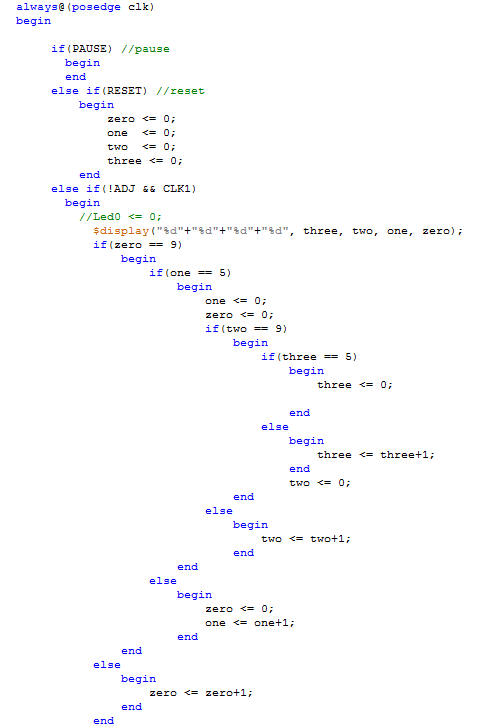
\includegraphics[scale=0.6]{topmod1}
	\caption{\textbf{Figure 1: Top module case-based counter implementation.}}
\end{figure}
The above figure shows the top module implementation of a case-based counter by check BCD values for edge cases and taking care of the specific circumstances, such as incrementing the next-most significant digit and setting the current digit back to zero. The block of code shown above has a check for a CLK1 high in order to handle the case where adjust is off. CLK1 was changed from a 50\% duty cycle clock into this pulse because this check would execute many consecutive times rather than just on one period of the 1Hz clock because the always@ block is triggering on the 100MHz reference clock. A similar approach was taken to create the adjust mode case, which is shown in the figure below.

\begin{figure}[H]
	%\hspace*{-1cm}
	\centering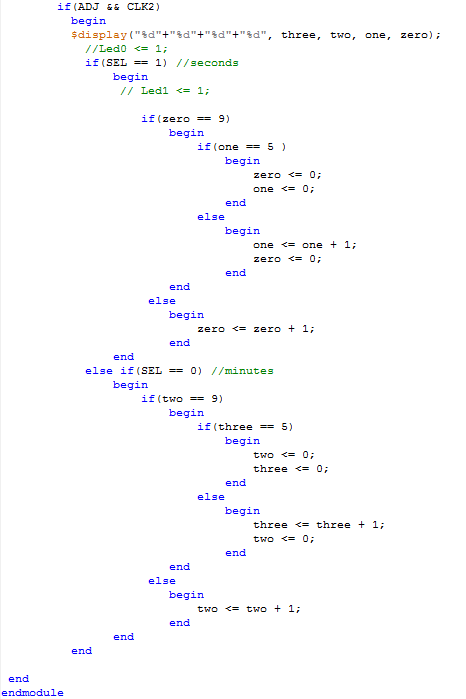
\includegraphics[scale=0.6]{topmodsel}
	\caption{\textbf{Figure 2: Top module case-based counter implementation showing the second part of the always@ block, where the ADJ HIGH case is taken into account.}}
\end{figure}
The same thing was done to take care of the 2Hz incrementing when ADJ is logic HIGH. The 2Hz signal was a pulse rather than a 50\% duty cycle clock. The inputs and outputs are:
\begin{enumerate}
	\item input CLK\_REF: This is the 100MHz reference clock from the FPGA fed in from the top module.
	\item input CLK\_RES: This is a reset signal fed in from the top module. It sets the state of both CLK1 and CLK2 to be low and sets the counter equal to zero.
	\item output reg CLK\_2HZ: This is the CLK2, 2Hz pulse signal used for incrementing when the ADJ value is high.
	\item output reg CLK\_1HZ: This is the CLK1, 1Hz pulse signal used for incrementing when the ADJ value is low.
\end{enumerate}
The code for the clock module included in "clock.v" is shown below.
\begin{figure}[H]
	%\hspace*{-1cm}
	\centering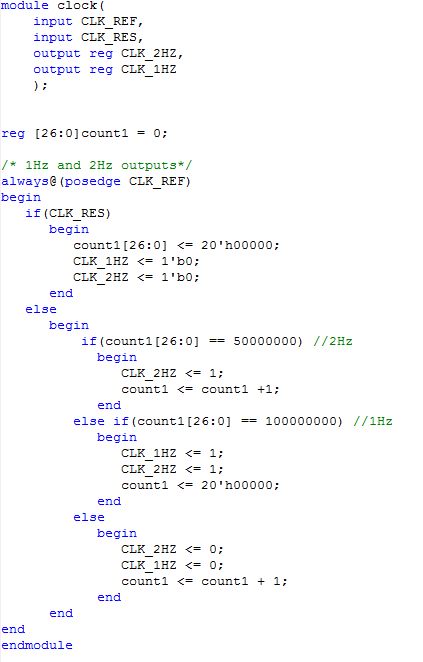
\includegraphics[scale=0.6]{clockmod}
	\caption{\textbf{Figure 3: Code block showing the clock module implementation with the pulse-based counters.}}
\end{figure}
Our module requires only one counter, and we rely on clock division of the 100MHz clock to check for specific cases in order to set the pulses equal to HIGH for one cycle of the 100MHz clock.




\subsection{Display Module}
The seven-segment display can only display one number between zero and nine across all digits at one time, so multiplexing the digits at a relatively high frequency is required to create the illusion of digit stability and make it appear as if the digits are different. 
\par
The module inputs and outputs are:
\begin{enumerate}
	\item input CLK: This is the 100MHz reference clock from the FPGA used for edge triggering.
	\item input CLK1: 1Hz clock input.
	\item input CLK2: 2Hz clock input.
	\item input ADJ:  Adjustment input from top module.
	\item input SEL:  Selector input to be used when ADJ is HIGH.
	\item input RESET: The reset signal comes from the user pressing the reset button. This will set the digit to display equal to zero from within this module and for the duration of the reset signal display a blank value.
	\item input [3:0] d0, d1, d2, d3: These 4-bit regs correspond to the zero, one, two, and three digit positions from the top module. The multiplexed digit will be set to one of these four values depending on the state.
	\item output reg[6:0] dispDigit: This 7-bit reg includes all of the values to display a digit on the seven segment display.
	\item output reg[3:0] selector: The selector determines which of the digits will be selected to display.
\end{enumerate}
We moved the fast clock into the display module since it was counter based and it made more sense to make it local. 
\begin{figure}[H]
	%\hspace*{-1cm}
	\centering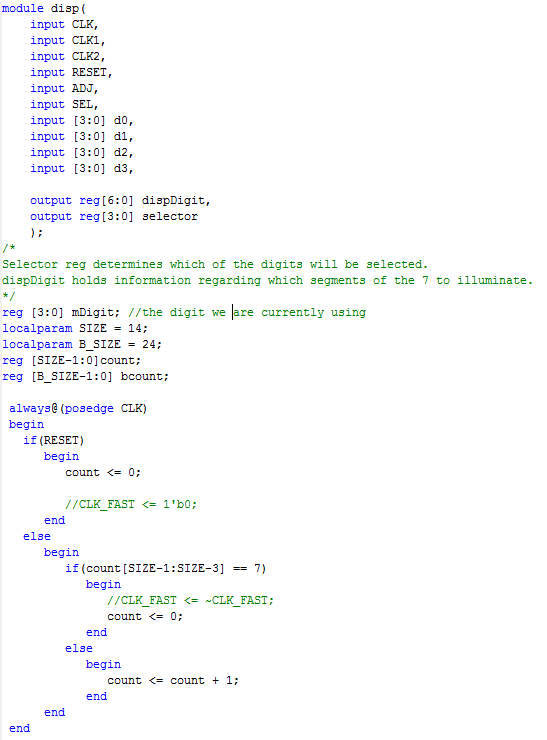
\includegraphics[scale=0.6]{clkfast}
	\caption{\textbf{Figure 4: Local implementation of the fast clock used for display multiplexing.}}
\end{figure}

The counter variable used in this clock was also used to decide which digit to select in the multiplexer. Bits MSB and MSB-1 can be viewed as providing four possible cases: 00, 01, 10, 11. These cases were checked for on each rising edge of the 100MHz clock and a corresponding digit was selected.
\begin{figure}[H]
	%\hspace*{-1cm}
	\centering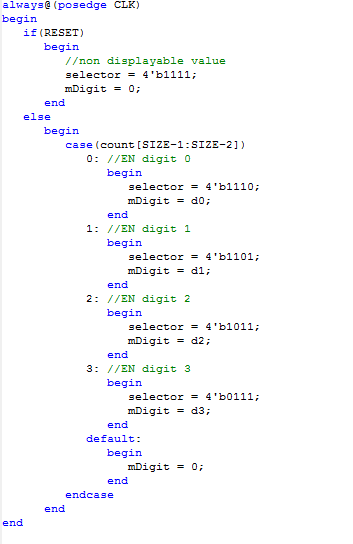
\includegraphics[scale=0.6]{counterchk}
	\caption{\textbf{Figure 5: Using the fast clock's counter MSB and MSB-1 as the conditions for changing state.}}
\end{figure}
Finally, whenever the multiplexed digit "mDigit" was changed, the value of dispDigit was updated with the new value. This is shown in the image below:
\begin{figure}[H]
	%\hspace*{-1cm}
	\centering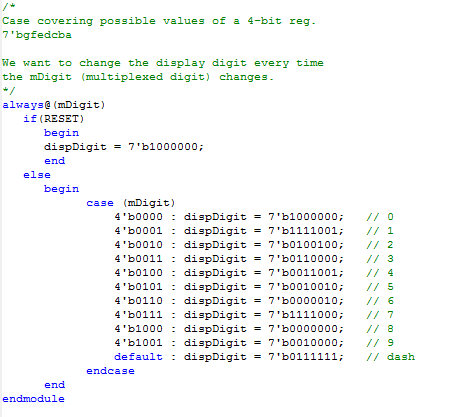
\includegraphics[scale=0.6]{changedisp}
	\caption{\textbf{Figure 6: Switching on the value of mDigit to update dispDigit accordingly. Recall dispDigit is the 7-bit output that corresponds to which parts of the display to light up.}}
\end{figure}
By tweaking the value of the localparam SIZE, we were able to change the speed of the clock. Smaller values SIZE will mean that the cases are reached more quickly, whereas larger values will make the clock slower.
\par
The blinking was triggered when ADJ was set to HIGH. The selector switch SEL denoted whether minutes or seconds would blink. To make the blinking, we held the opposite two digits at the high frequency of ran the digits of interest at a lower frequency. This code took many lines and can be viewed in the source code for "disp.v."
\subsection{Counter Module}
We initially created mod-6 and mod-10 counters in a file called "counter.v" for use in providing the digit counting functionality. However, we decided that it was simpler to check BCD states in the top module and handle special cases (when fives and nines occur in upper and lower digits respectively.) This resulted in an easy to implement solution but it isn't very clean and takes up many lines.
\subsection{Stopwatch Module (Top Module)}
The top module "SW.v" brings together all of the submodules and implements both the adjustment and selector features. The inputs and outputs are defined as follows:
\begin{enumerate}
	\item input clk: 100MHz reference clock from the FPGA. This gets passed into the instantiation of the clock module as well as the display module.
	\item input RESET: Reset signal coming from a button specified in the ucf file. Passed into both sub-modules.
	\item input PAUSE: Pause signal coming from a button specified in the ucf file. Passed into both sub-modules.
	\item input ADJ: The adjustment signal that denotes whether or not the clock should go into adjust mode. This also comes from a button specified in the ucf file.
	\item input SEL: The selector signal that specifies the which set of digits to increment when ADJ is set to HIGH. 
	\item output[6:0] dispDigit: 7-bit output reg that is updated by the display module.
	\item output[3:0] selector: 4-bit output reg that is updated by the display module and denotes how to light up digits.
\end{enumerate}
Figure 2. shows the second part of the top module's always@ block. This portion deals with the case where ADJ is HIGH. The clock should be incremented at 2Hz, so there is also an AND check for CLK2 being HIGH as well. The cases for SEL = 1 or SEL = 0 include incrementing for either the zero or the two digit respectively.  
\par
Adding this to the top module was not the cleanest way, because code was duplicated and we never ended up using our counter module. 
\begin{figure}[H]
	%\hspace*{-1cm}
	\centering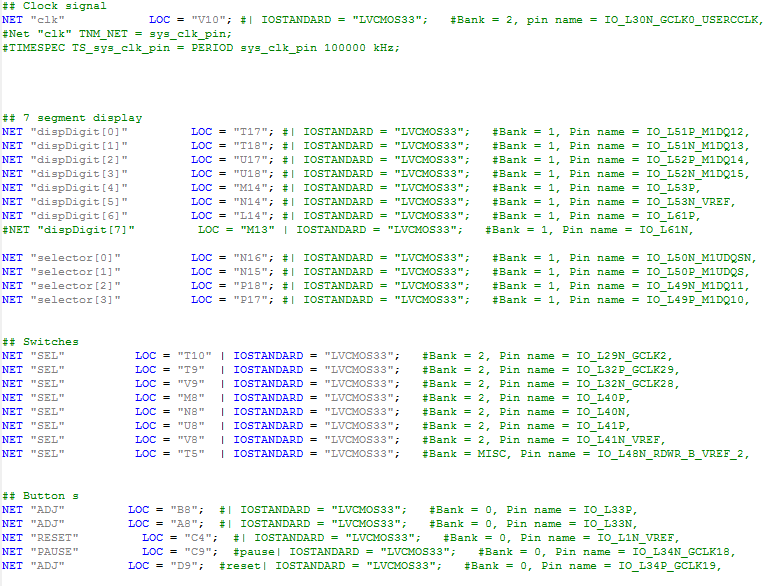
\includegraphics[scale=0.5]{ucf}
	\caption{\textbf{Figure 7: The UCF file specifying how pins were connected to inputs and outputs in the modules.}}
\end{figure}
The UCF file from lab 1 was modified and changed to suit our design. We noticed through iterative testing that certain buttons and slider switches were more receptive of assignments than others, so the settings displayed above were the optimal ones. 

\section{Simulation Documentation}
We used the simulator to test basic functionality of our counter and clocks. We checked to make sure that the counters were setting that carry out and main regs accordingly at their respective mod values, despite not using the counter in our final implementation. We verified that the clock pulses were appearing at the right time stamps. 
\par
Rather than looking at solely waveforms, we added \$display statements in the top module where the counter is implemented in order to see the minutes and seconds increment. Since the simulator takes a long time to simulate on the order of seconds, we triggered each counter on the 100MHz clock to speed things up. This allowed us to verify the carry behavior for cases such as xx:x9, x9:x9, x9:59, and 59:59.
\par 
Once we confirmed that everything was working as expected, we created a programming file and tested on the FPGA. The only difficulty that came with working with the hardware was getting the buttons to work properly. Some buttons on the nexsys3 board just weren't receptive of input.
\par
For reference, the test bench files are included with the project zip file turned in.

\section{Conclusion}
The goal of this project was to create a modular solution to a simple problem that required careful consideration of boundary cases and timing. The trials encountered in this lab further reinforced the idea that timing is everything with digital logic. Clock errors and triggering on the wrong clock caused us issues with the counters. This was fixed by looking at waveforms and time stamps in the simulator.
\par 
One difficulty was implementing blinking. This required holding two digits constant while the others blinked and the LSB of the subset incremented at 2Hz. We needed to add a separate counter "bcount" withint the display module in order to create different updating speeds in the case statement.  
\par
The process to go from code to hardware was very straightforward. The UCF file allows pin designators to be tied to the inputs and outputs of the top module, so we just renamed the specific pins we needed to use.
\par
Our design could be improved in the future by using the counter module rather than having it integrated into the top module. 



\end{document}

